\documentclass[12pt]{article}
\usepackage[english]{babel}
\usepackage[utf8]{inputenc}

%% Pointer to 'default' preamble
% pacakages and definitions

\usepackage{geometry}
\geometry{
	letterpaper, 
	portrait, 
	top=.75in,
	left=.8in,
	right=.75in,
	bottom=.5in		} 	% Page Margins
	
%% additional packages for nice things
\usepackage{amsmath} 	% for most math
\usepackage{commath} 	% for abs
\usepackage{lastpage}	% for page count
\usepackage{amssymb} 	% for therefore
\usepackage{graphicx} 	% for image handling
\usepackage{wrapfig} 	% wrap figures
\usepackage[none]{hyphenat} % for no hyphenations
\usepackage{array} 		% for >{} column characterisctis
\usepackage{physics} 	% for easier derivative \dv....
\usepackage{tikz} 		% for graphic@!
\usepackage{circuitikz} % for circuits!
\usetikzlibrary{arrows.meta} % for loads
\usepackage[thicklines]{cancel}	% for cancels
\usepackage{xcolor}		% for color cancels
\usepackage[per-mode=fraction]{siunitx} % for si units and num
\sisetup{group-separator = {,}, group-minimum-digits = 3} % additional si unit table functionality

\usepackage{fancyhdr} 	% for header
\usepackage{comment}	% for ability to comment out large sections
\usepackage{multicol}	% for multiple columns using multicols
\usepackage[framed,numbered]{matlab-prettifier} % matlab sytle listing
\usepackage{marvosym} 	% for boltsymbol lightning
\usepackage{pdflscape} 	% for various landscape pages in portrait docs.
%\usepackage{float}
\usepackage{fancyvrb}	% for Verbatim (a tab respecting verbatim)
\usepackage{enumitem}	% for [resume] functionality of enumerate
\usepackage{spreadtab} 	% for using formulas in tables}
\usepackage{numprint}	% for number format in spread tab
\usepackage{subcaption} % for subfigures with captions
\usepackage[normalem]{ulem} % for strike through sout

% for row colors in tables....
\usepackage{color, colortbl}
\definecolor{G1}{gray}{0.9}
\definecolor{G2}{rgb}{1,0.88,1}%{gray}{0.6}
\definecolor{G3}{rgb}{0.88,1,1}

% For table formatting
\usepackage{booktabs}
\renewcommand{\arraystretch}{1.2}
\usepackage{floatrow}
\floatsetup[table]{capposition=top} % put table captions on top of tables

% Caption formating footnotesize ~ 10 pt in a 12 pt document
\usepackage[font={small}]{caption}

%% package config 
\sisetup{output-exponent-marker=\ensuremath{\mathrm{E}}} % for engineer E
\renewcommand{\CancelColor}{\color{red}}	% for color cancels
\lstset{aboveskip=2pt,belowskip=2pt} % for more compact table
%\arraycolsep=1.4pt\def
\setlength{\parindent}{0cm} % Remove indentation from paragraphs
\setlength{\columnsep}{0.5cm}
\lstset{
	style      = Matlab-editor,
	basicstyle = \ttfamily\footnotesize, % if you want to use Courier - not really used?
}
\renewcommand*{\pd}[3][]{\ensuremath{\dfrac{\partial^{#1} #2}{\partial #3}}} % for larger pd fracs
\renewcommand{\real}[1]{\mathbb{R}\left\{ #1 \right\}}	% for REAL symbol
\newcommand{\imag}[1]{\mathbb{I}\left\{ #1 \right\}}	% for IMAG symbol
\definecolor{m}{rgb}{1,0,1}	% for MATLAB matching magenta
	
%% custom macros
\newcommand\numberthis{\addtocounter{equation}{1}\tag{\theequation}} % for simple \numberthis command

\newcommand{\equal}{=} % so circuitikz can have an = in the labels
\newcolumntype{L}[1]{>{\raggedright\let\newline\\\arraybackslash\hspace{0pt}}m{#1}}
\newcolumntype{C}[1]{>{\centering\let\newline\\\arraybackslash\hspace{0pt}}m{#1}}
\newcolumntype{R}[1]{>{\raggedleft\let\newline\\\arraybackslash\hspace{0pt}}m{#1}}

%% Header
\pagestyle{fancy} % for header stuffs
\fancyhf{}
% spacing
\headheight 29 pt
\headsep 6 pt

%% Header
\rhead{Thad Haines \\ Page \thepage\ of \pageref{LastPage}}
\chead{Comparison of DC simulation results \\ between PST versions 2.3, 3.1, and SETO}
\lhead{Research \\ 7/14/20}

\usepackage{minted}
\usepackage{setspace}
\usepackage{lscape}
\usepackage{multicol}
\begin{document}
\onehalfspacing
\paragraph{Summary}
\begin{itemize}
\item A HVDC case has been created and tested as working in all versions of PST. 
\item Using the structured global approach increases speed by over 2 times.
\item Minor differences exist between version 2.3 and 3.1 in non-linear simulation output.
\item All linear results match between versions, but do not match non-linear output (possibly due to improper data handling).
\end{itemize}

\paragraph{Scenario Description} \ \\
A 16 bus system with one HVDC link and four machines equipped with st3 exciters, pss, and governors was perturbed by a 0.1 PU active load pulse from $t=1$ to $t=2$

\paragraph{Non-Linear Results} \ \\
The new pstSETO version is based on version 3.1 so it makes sense that there are no differences in machine speed or bus voltage and angle.
However, total non-linear simulation time in 3.1 is 18.876 seconds, while pstSETO only takes 8.853 seconds.

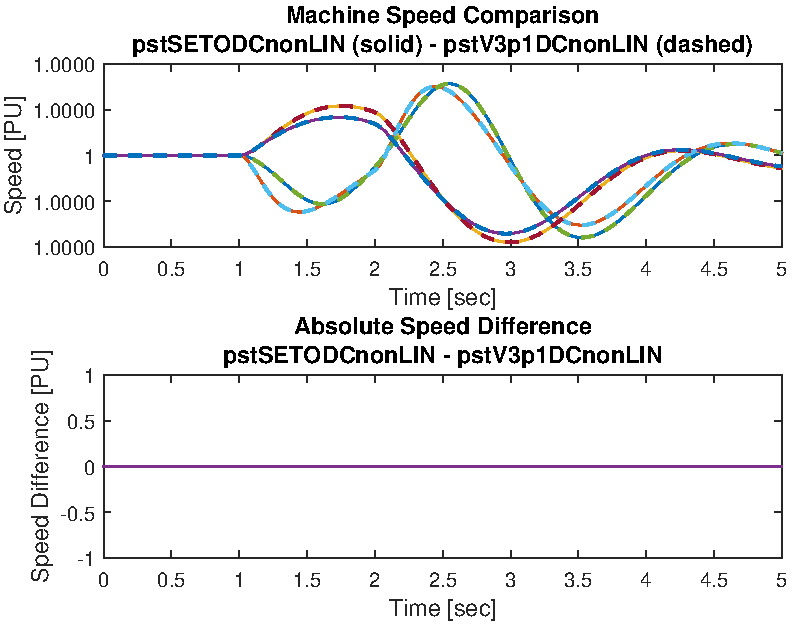
\includegraphics[width=.3\linewidth]{pstSETODCnonLINpstV3p1DCnonLINMacSpd} %
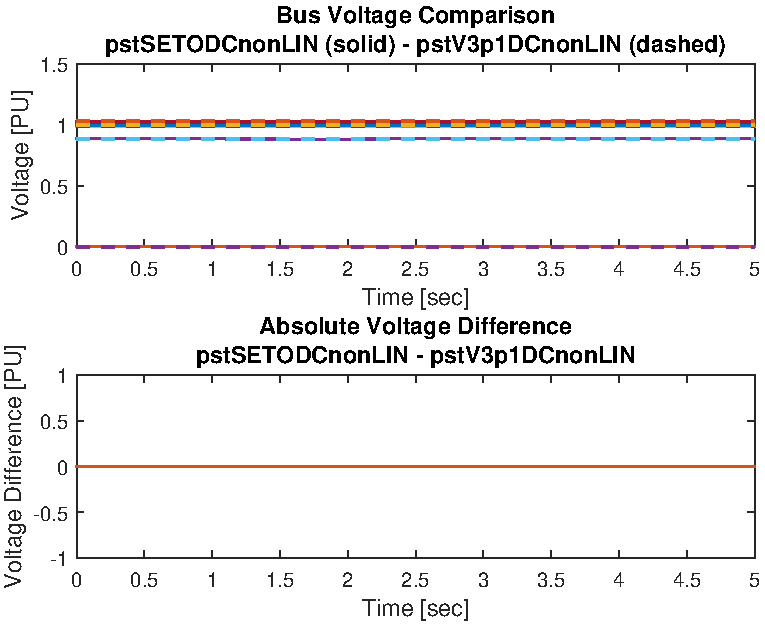
\includegraphics[width=.3\linewidth]{pstSETODCnonLINpstV3p1DCnonLINBusV} %
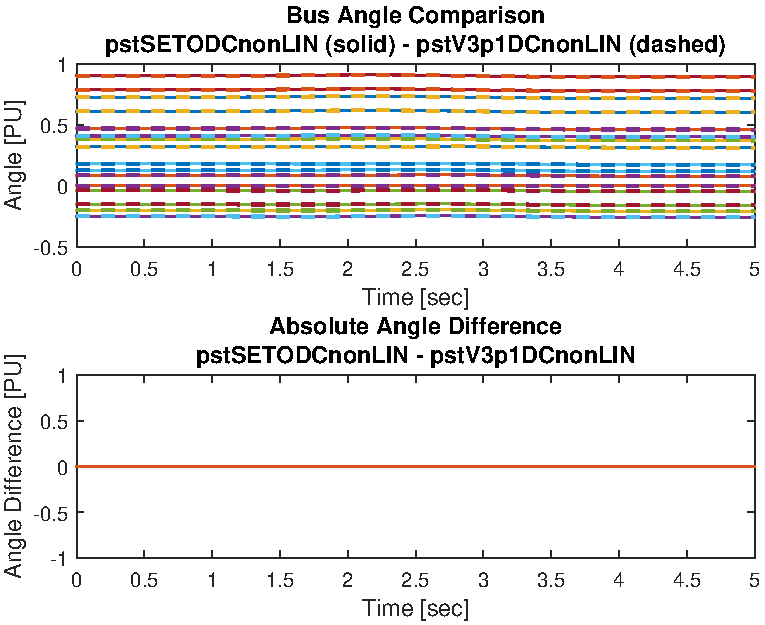
\includegraphics[width=.3\linewidth]{pstSETODCnonLINpstV3p1DCnonLINAngle} \\

The differences between version 3.1 and 2.3 range between  $10^{-11}$ to $10^{-9}$.
Judging from the initial difference, there must have been changes to the way DC lines were initialized between version 2 and 3.

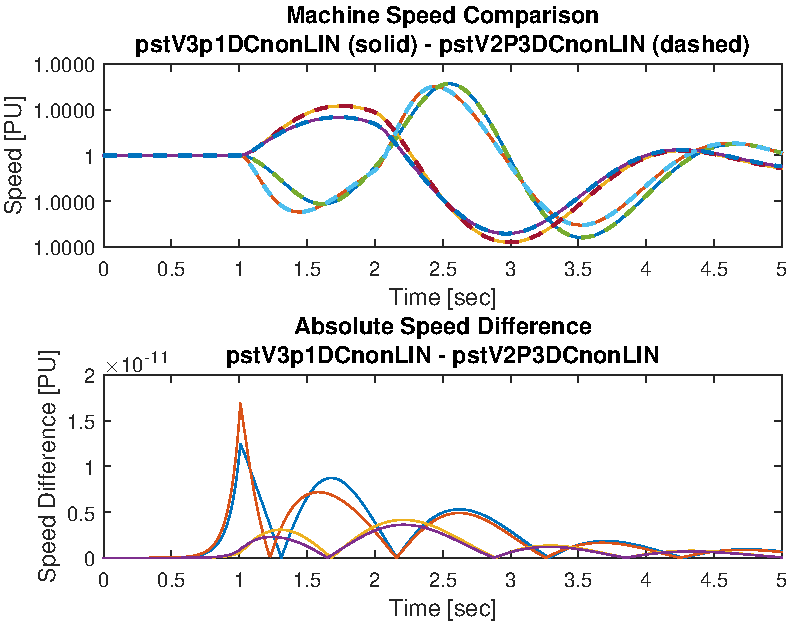
\includegraphics[width=.3\linewidth]{pstV3p1DCnonLINpstV2P3DCnonLINMacSpd} %
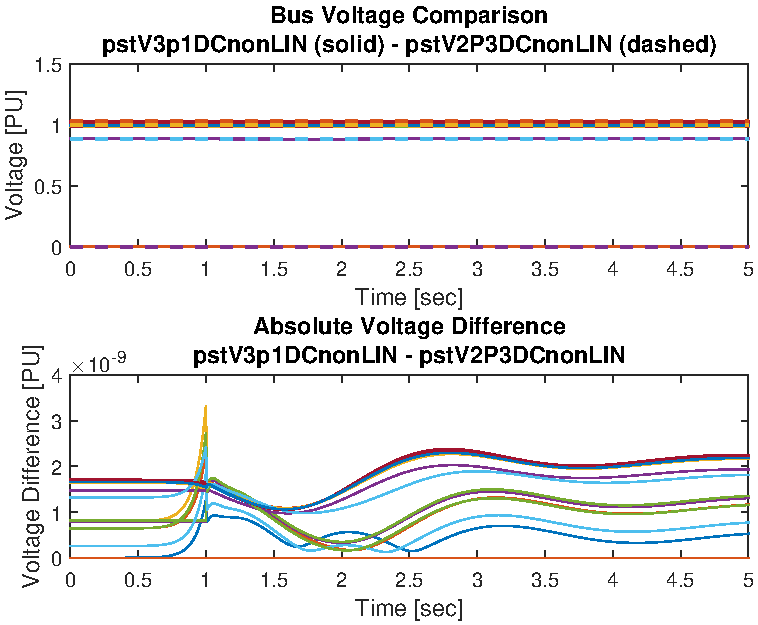
\includegraphics[width=.3\linewidth]{pstV3p1DCnonLINpstV2P3DCnonLINBusV} %
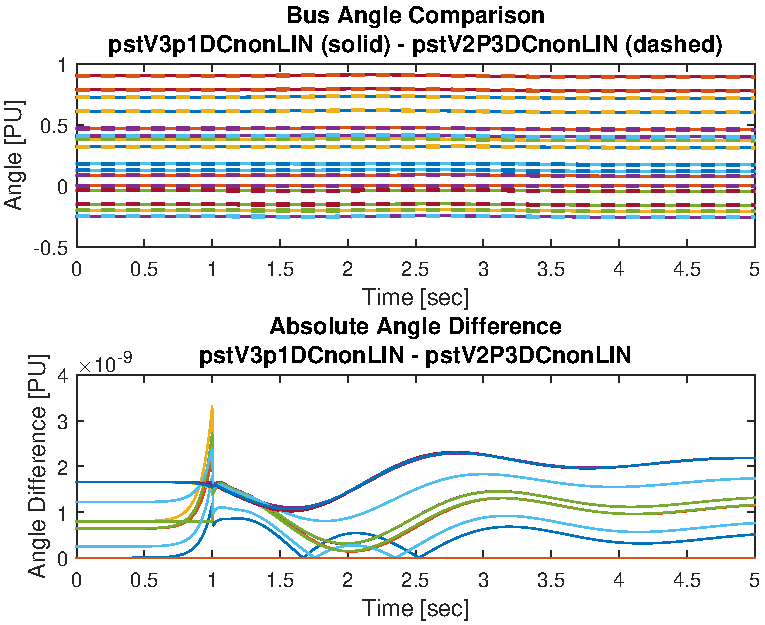
\includegraphics[width=.3\linewidth]{pstV3p1DCnonLINpstV2P3DCnonLINAngle} \\

\paragraph{Linear Results} \ \\
All versions provide the same output, however it does not match non-linear data.
This is very possibly due to improper data handling.

\end{document}
